Finally, we examine performance of a Machine Learning (ML) algorithms. 
The goal of this experiment is to evaluate better memory management strategies in ML algorithms developed with Rust.
We employ K-Nearest-Neighbors (KNN) for ML algorithm to be studied in our experiments.
Our KNN algorithms perform document classification on Wikipedia page data set described in Section~\ref{sec:eval_setdetail}. 

The algorithms have 4 phase; load, preprocess, query, and combine phase. 
Before these phase, we separate data sets into 8 partitions to run these in different threads. 
The algorithms spawn threads at the beginning ,and in the load phase partition of files are loaded in each threads. 
In preprocessing phase, the algorithm process document strings to generate Term-frequencies (Tfs) matrices and other data structures. 
In query phase, it calculates cosine similarities between all combination of train and test observations and select to top \(K\) nearest neighbors. 
In combine phase, the results from each batch and from each are combined. 
Based on our experiments result, the runtime in preprocess and query phase are significantly larger than other two phases.
Therefore, we focus discussion in these two phases considering them bottlenecks in our KNN algorithms.

KNN algorithms are implemented with different memory management strategies. 
We parametrize these memory management and some other values. These parameters are listed in Table~\ref{tab:parameter}. 

\begin{table}
    \renewcommand{\arraystretch}{1.2}
    \begin{tabular}{|l|l|l|l|l|}
    \hline
    Parameter Name  & \multicolumn{4}{l|}{Values and Description}                                                                                                                                                                                \\ \hline
    Method          & \multicolumn{4}{l|}{\begin{tabular}[c]{@{}l@{}}deep-copy:  use deep-copy to generate intermediate objects\\ arc: use atomic reference count to generate intermediate objects\end{tabular}}                                 \\ \hline
    Strategy        & \multicolumn{4}{l|}{\begin{tabular}[c]{@{}l@{}}1: keep intermediate objects in memory until owner is changed\\ 2: remove intermediate objects as soon as it is not needed\end{tabular}}                                    \\ \hline
    Number of batch & \multicolumn{4}{l|}{\begin{tabular}[c]{@{}l@{}}2: generate 2 batches from each partition\\ 3: generate 3 batches from each partition\end{tabular}}                                                                             \\ \hline
    k               & \multicolumn{4}{l|}{\begin{tabular}[c]{@{}l@{}}15K: dimension of feature matrices is 15 thousands \\ 20K: dimension of feature matrices is 20 thousands\\ 25K: dimension of feature matrices is 25 thousands\end{tabular}} \\ \hline
    \end{tabular}
    \caption{Parameter of KNN algorithms}
    \label{tab:parameter}
 \end{table}


Method parameter is specified to select memory management strategy used in preprocess phase. 
In preprocess phase, the algorithm generates many intermediate data structures using same String elements.
Deep-copy method deeply copies String to generate intermediate data structures. Arc method use Atomic Reference Count (Arc) to wrap String elements in the original data structure and 
clone Arc when the elements are used in other data structures. As Experiment 4 had shown in in Section~\ref{sec:eval_treeagg}, deep-copy of complex objects is more expensive than cloning Arc. 
String is a sort of objects allocated in heap and copied many times in preprocess phase. Therefore, it is worth to assess which method can be better memory management strategy in our experiments.

Strategy parameter controls memory management strategy used in both preprocess and query phase.
Strategy 1 keeps all intermediate data structures and numeric matrix objects from preprocess to query phase. 
Strategy 2 removes these data structures and objects as soon as they are not needed. 
These strategies differ from each other in terms of memory usage and frequency of memory deallocations.
These may cause significant runtime difference of the algorithms.

Number of batch controls number and size of batch for each partition. This parameter varies size of intermediate data structures and numeric matrices, and 
frequency of memory deallocations. 
The size of each batch is defined in 6250 pages when we have 2 batches, and 4166 or 4167 when we have 3 batches. 
The parameter k specifies number of dimension of feature matrices created out of preprocess phase. 
By controlling this, it determines size of intermediate data structures and numeric matrices. 

By controlling these parameter, we compare runtime and memory usage of KNN algorithms. 


\subsection{Result}
\label{sec:history}
Figure~\ref{fig:total}, ~\ref{fig:preprocess}, and ~\ref{fig:query} show the runtime performance of our KNN algorithms in total, preprocess, and query phase respectively. 
The algorithms used in our experiments are indexed in Table~\ref{tab:algorithm}. We call each algorithm in algorithm number for easy understanding.
The Algorithm 3 with 20K and 25K dimension, and the Algorithm 1 with 25K dimension whose runtime is showing 0 seconds are algorithms that are terminated during execution due to fail of memory allocation.

Figure~\ref{fig:total} shows Algorithm 8 shows much slower performance compare to the other algorithms.
Algorithm 7 also starts to slow down as we increase the number of dimension.  

As shown in Figure~\ref{fig:preprocess}, the algorithms using Arc is much slower than using deep-copy in preprocessing phase. 
Algorithm 6 is 38\%  slower than Algorithm 6 in dimension of 25K. 
In addition, the algorithms with strategy 2 are slower than with strategy 1. 
For example, Algorithm 6 is about 85\% slower than one Algorithm 2 in dimension of 25K.
The algorithms with 3 batches are slower that ones with 2 batches. Furthermore, as we increase the number of dimension, the number of batch becomes more and more critical to runtime performance of the algorithms with deep-copy.
The runtime ratios of difference from Algorithm 7 to Algorithm 8 are about 44\%, 28\%, and 39\% for dimension of 15K, 20K, and 25K respectively. 
However, those from Algorithm 5 to Algorithm 6 are about 11\%, 28\%, and 54\%. The ratios of difference increase proportionally to the number of dimension. 

In query phase, Algorithm 8 is much slower than the others in different parameter settings.
Algorithm 7 starts to slow down as number of dimension is increased. 


\begin{table}
    \renewcommand{\arraystretch}{1.2}
    \begin{tabular}{|l|l|l|l|}
    \hline
    Algorithm number & Method    & Strategy & Number of batch \\ \hline
    1                & deep-copy & 1        & 2               \\ \hline
    2                & deep-copy & 1        & 3               \\ \hline
    3                & arc       & 1        & 2               \\ \hline
    4                & arc       & 1        & 3               \\ \hline
    5                & deep-copy & 2        & 2               \\ \hline
    6                & deep-copy & 2        & 3               \\ \hline
    7                & arc       & 2        & 2               \\ \hline
    8                & arc       & 2        & 3               \\ \hline
    \end{tabular}
    \caption{Index of Algorithm}
    \label{tab:algorithm}
 \end{table}

\begin{figure}[htb]
    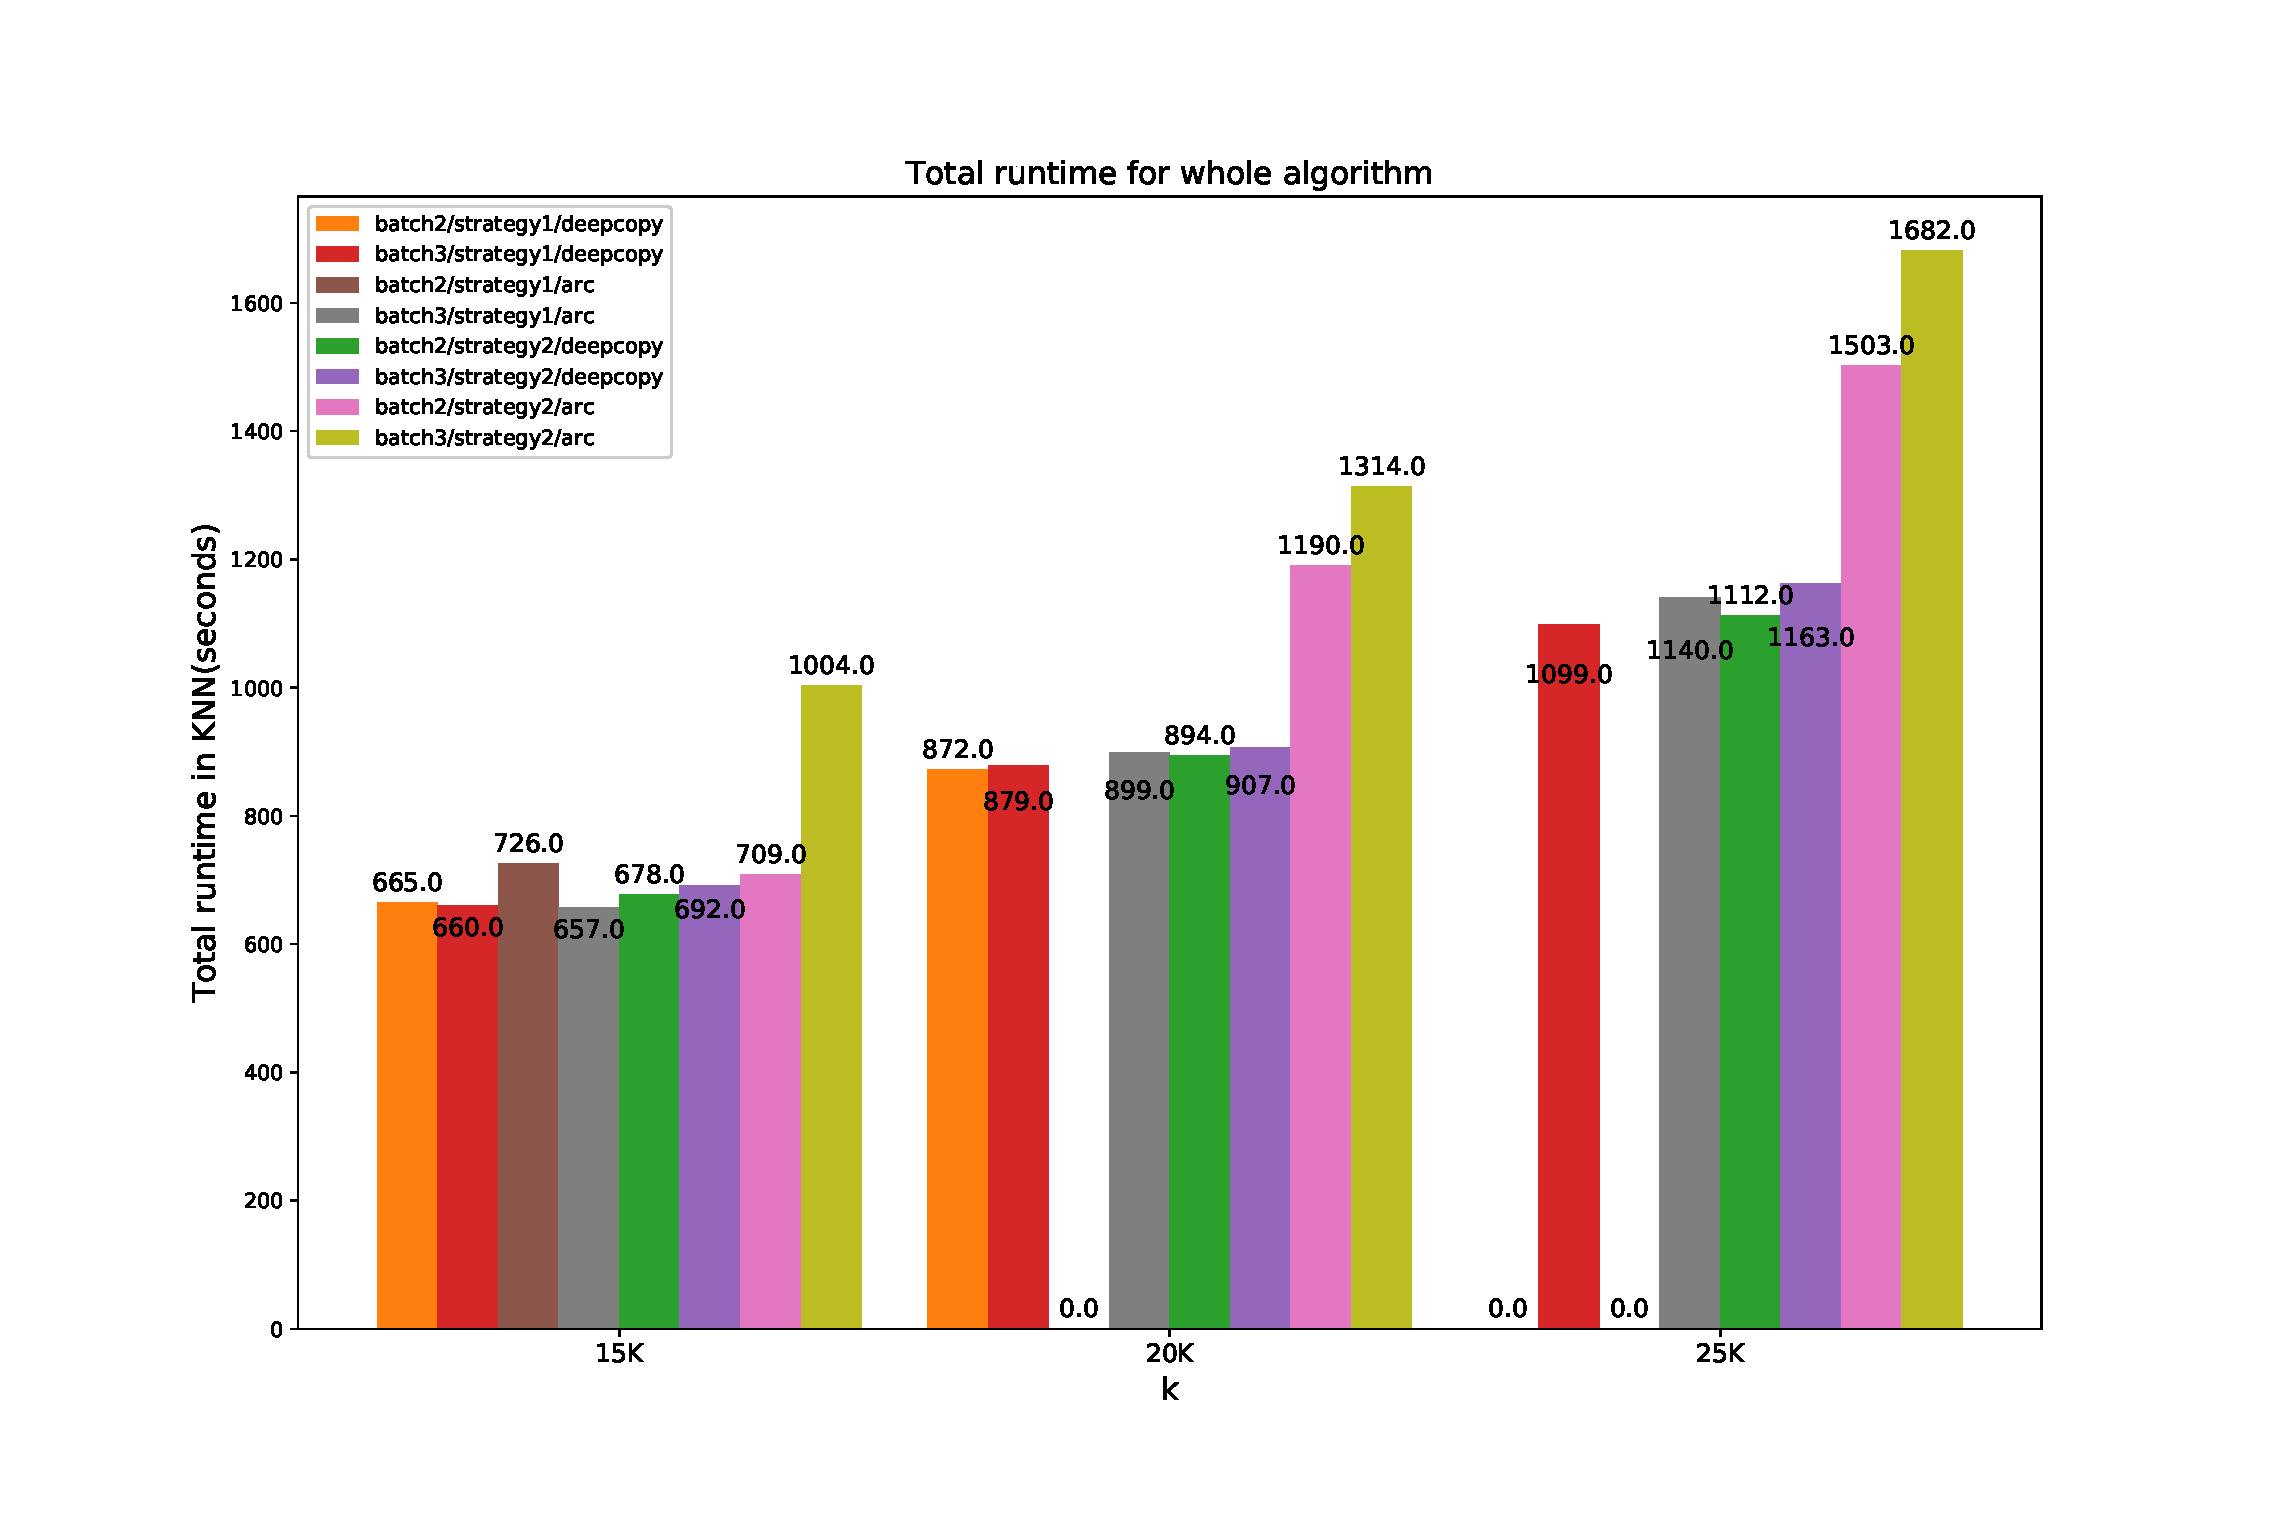
\includegraphics[width=15cm]{total.eps}
    \caption{Total runtime whole KNN algorithm (seconds)}
    \label{fig:total}
\end{figure}

\begin{figure}[htb]
    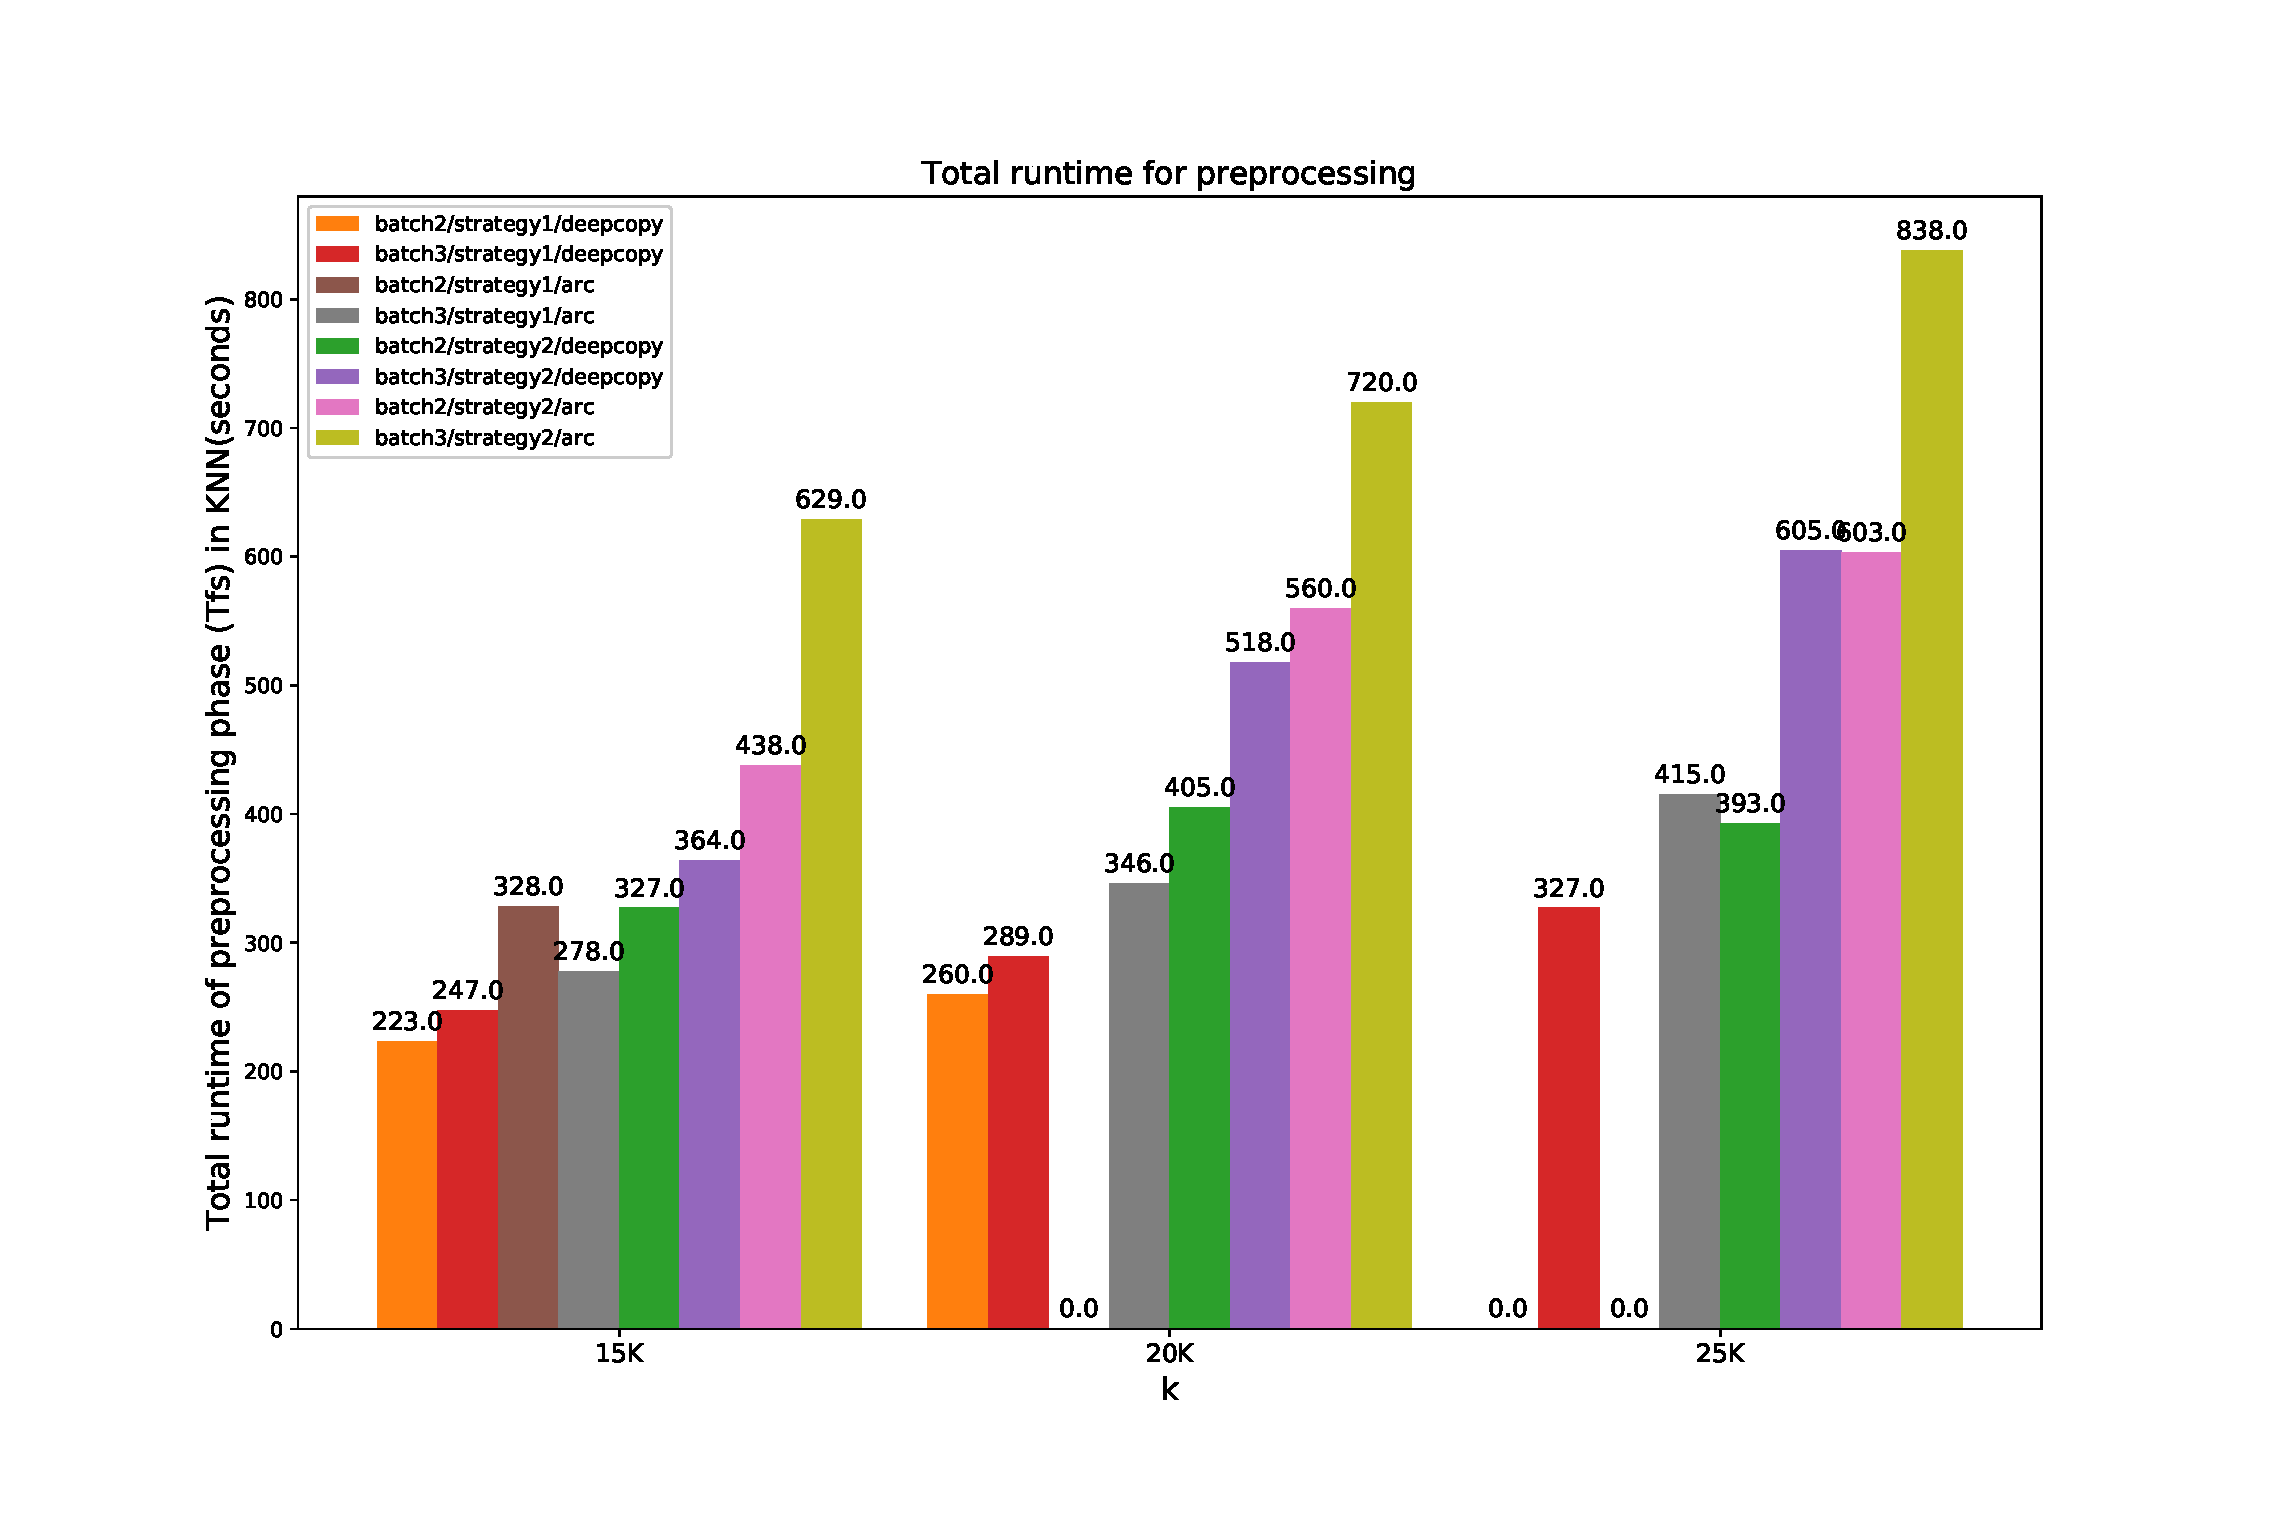
\includegraphics[width=15cm]{preprocessing.eps}
    \caption{Total runtime of preprocessing phase in KNN (seconds)}
    \label{fig:preprocess}
\end{figure}


\begin{figure}[htb]
    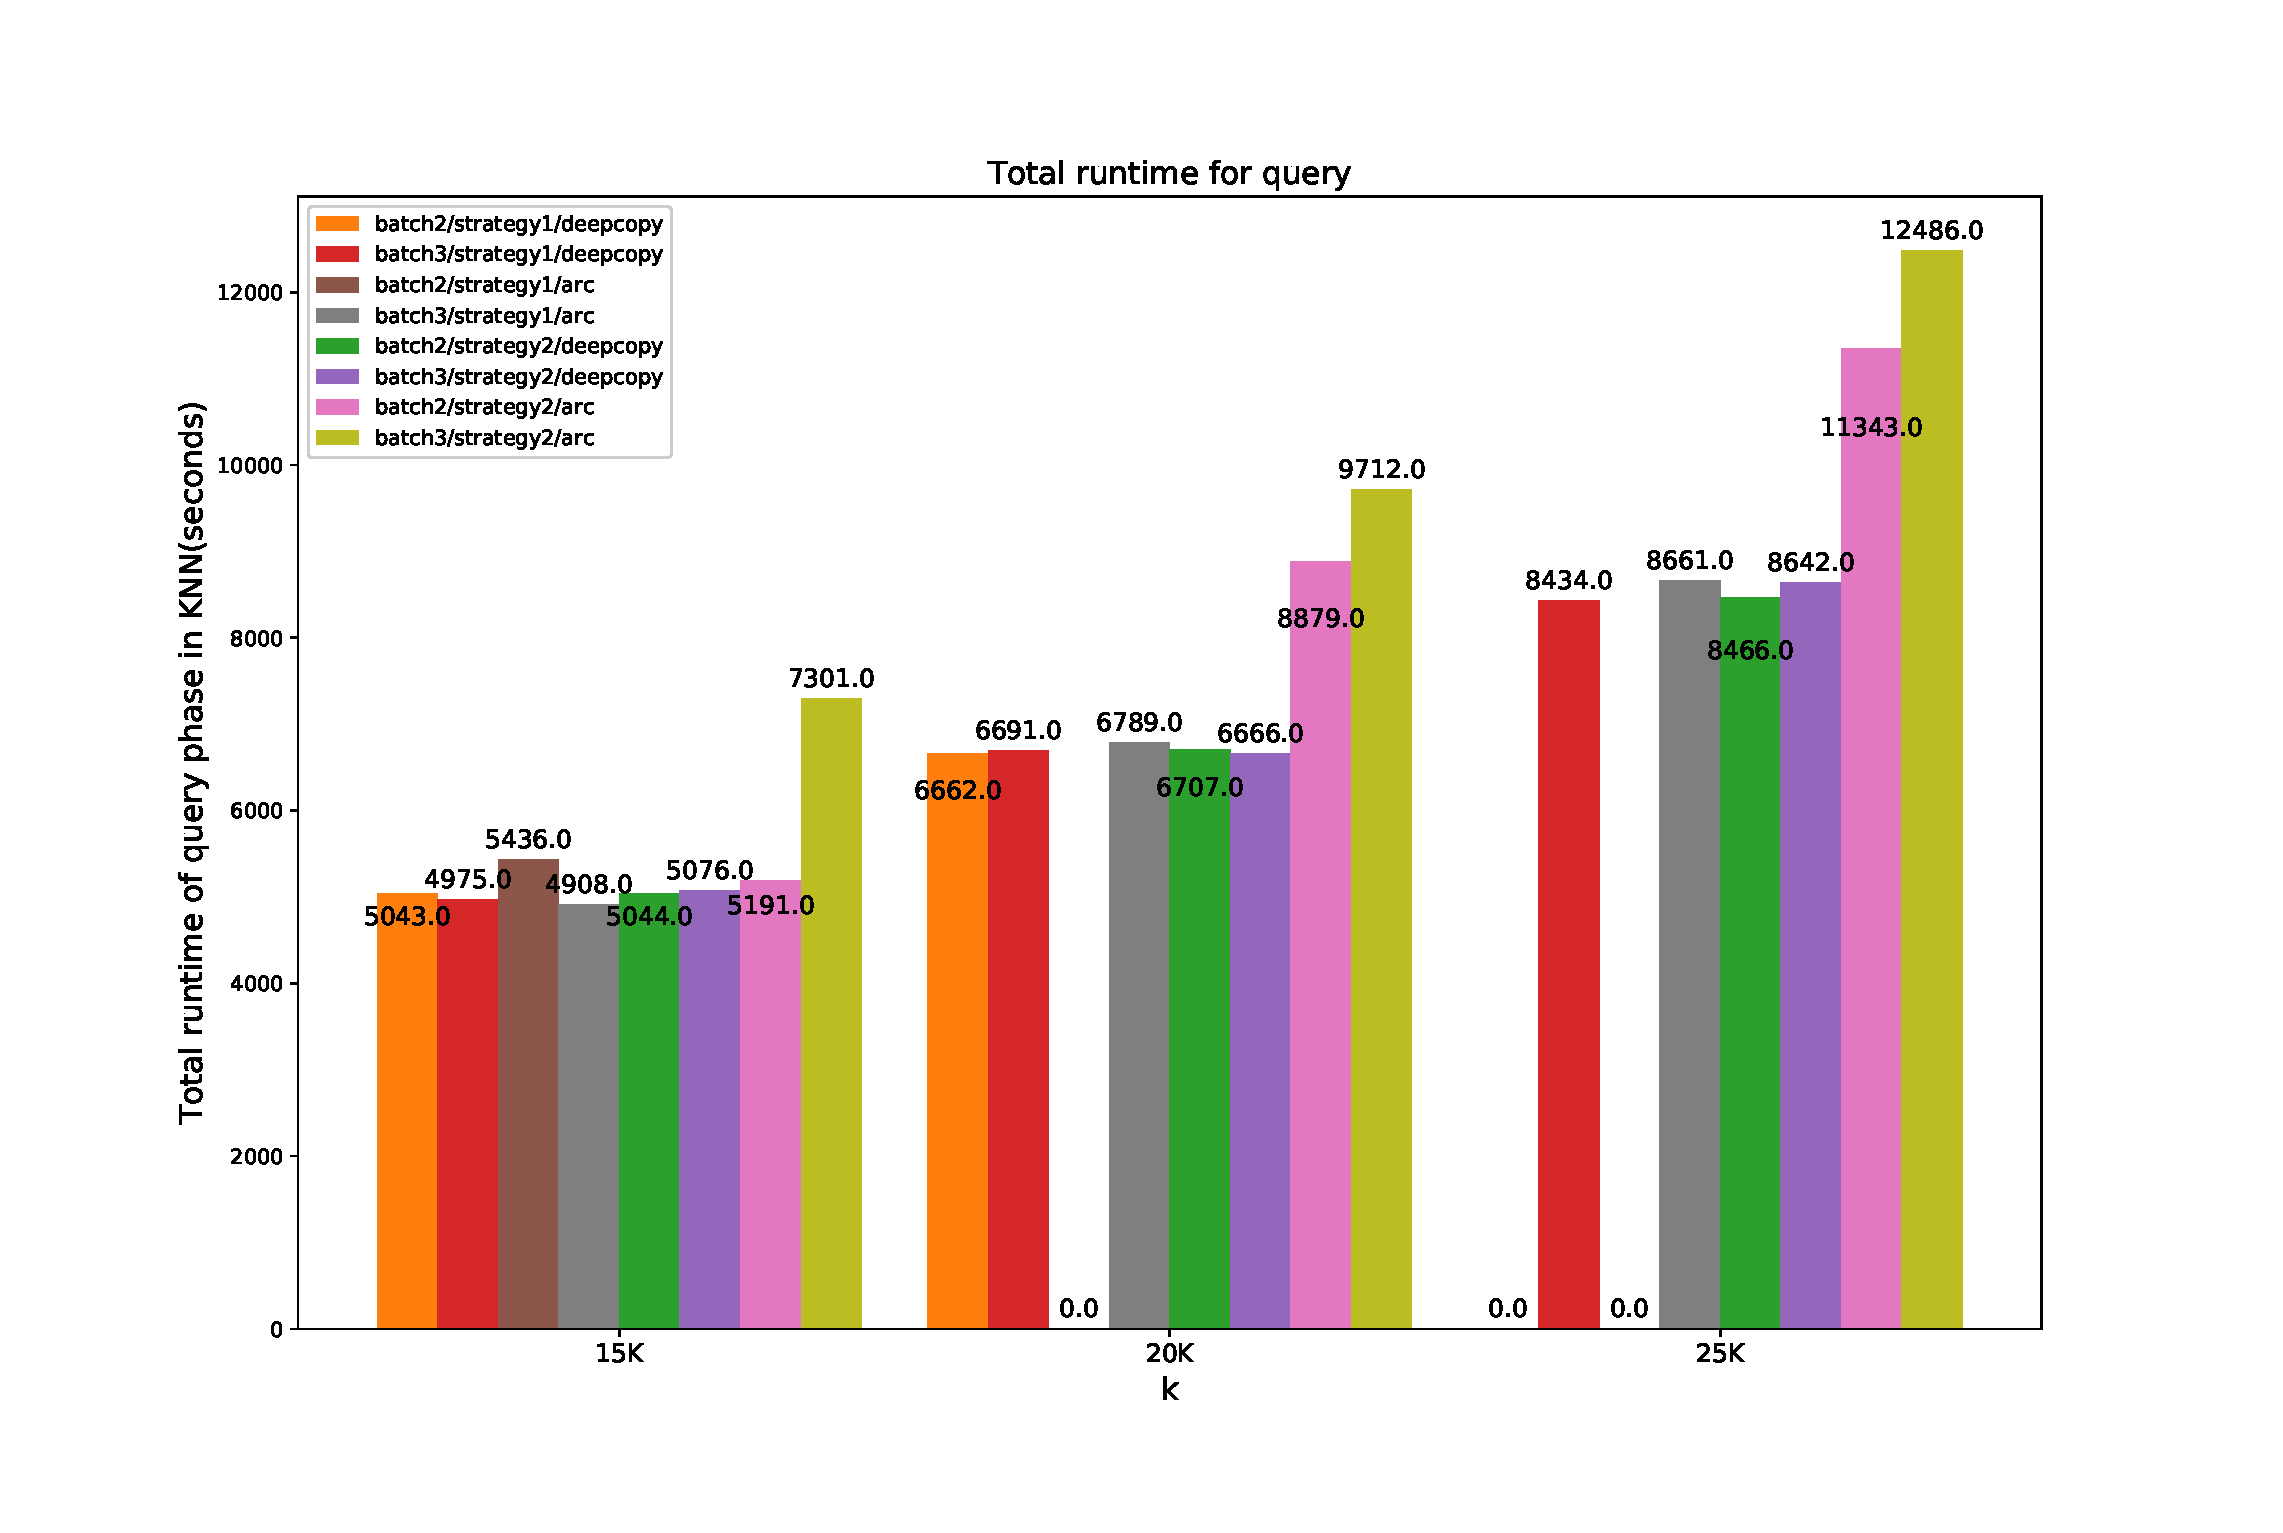
\includegraphics[width=15cm]{query.eps}
    \caption{Total runtime of query phase in KNN (seconds)}
    \label{fig:query}
\end{figure}


\subsection{Discussion}
\label{sec:history}
In preprocess phase, the algorithms using Arc method performs worse than ones with deep-copy method. 
This result may seem to contradict to the result of Experiment 4 in Section~\ref{sec:eval_treeagg}.
In Experiment 4, complex objects, CustomerOwned, are cloned with Arc or deep-copied. 
In this Experiment 5, we however get Arc or deep-copy of String instead of complex object.
The result explains deep-copying String is much inexpensive than deep-copying the complex object and 
using deep-copy method is actually efficient than using Arc to share String. 
Therefore, we need to make decision which method to use depending on size and complexity of objects.

In addition, use of different strategies in preprocess phase explains how deallocations of intermediate data structures and drops of their variables impact algorithm's runtime performance.
The result shows deallocations of intermediate data costs a lot; Algorithm 6 is 85\% slower than Algorithm 2.
This may be more severe bottleneck for algorithms using Arc; Algorithm 8 is 102\% slower than Algorithm 4.
This is the same reason explained in Experiment 4. 
Arc has to check reference count and its atomic operation is expensive. 

The impact of batch number can explain how frequency of memory de/allocation affects runtime performance. 
Dealing with more number of batch has negative impacts on runtime performance because it triggers more frequent memory de/allocation.
In addition, as we increase the number of dimension, the ration of runtime difference among different numbers of batch for the algorithms with deep-copy, but not for ones with Arc.
This is because algorithm with Arc does not de/allocate memory as much frequent as ones with deep-copy.
The intermediate data structures mealy get reference to String values without actually allocating memory for copied Strings.

In query phase, most of our algorithms shows similar runtime performance among the same number of dimension. 
Why such differences seen in preprocess phase are not shown in query phase? This is because the data structures processed in this phase are numeric matrices and vectors. 
These data structures do not contain String so that the selection of method parameter does not have direct impact to algorithm's runtime performance.

Furthermore, numeric matrices and vectors are contiguously allocated initializing their size, so they are easy to be de/allocated. 
The computation needed for these de/allocations is fairly fast. Therefore, setting parameters, such as number of batch and strategy, does not impacts runtime performance.

However, we can see significant degradation in Algorithm 7 with 20K and 25K dimension and Algorithm 8 with 15K, 20K, and 25K dimension. 
By using strategy 2, we deallocate the numeric matrices and vectors in query phase. However, it is difficult to think that these contiguous memory deallocations cause the degradation. 
If that is so, Algorithm 5 and 6 should also show some overheads. No page-swapping does not happen during the execution. 
One possible reason is that these algorithms suffer from the allocation of numeric matrices and vectors due to previous deallocation of intermediate data structures in preprocess phase. 
The frequent deallocations and low locality of Arc may lead long free-space-list making difficult to search enough spaces to allocate numeric matrices and vectors.
The other possibility is that the frequent deallocations and low locality of Arc cause cache of numeric matrices and vectors. 
The computation on these numeric objects may slow down due to their caching levels. 
To conclude these discussion, we need to conduct more experiments and deeper analysis. 
However, we push those discussion in next paper.

In a part of conclusion, using Arc to String may be overhead. Considered the result from Experiment 4, we need careful consideration which object to use which strategy, deep-copy and Arc.
In addition, frequent memory deallocation can lead to slower runtime performance. 
Therefore, we need to decide when to deallocate unused values taking account of memory capacity. 
